\newpage
\section{Scénario 2 : Chargement d'un script GraSyLa}
\label{sec:scenario2}

\subsection{Description et enjeux}
Ce scénario mesure les performances de chargement d'un script GraSyLa dans MetaDONE. Le script retenu pour les mesures est bpmn\_mm.grasyla, le méta-modèle BPMN fourni avec le plugin BPMN de MetaDONE. Il contient 106 équations et constitue un cas représentatif d'un script de taille réelle.

Le processus de chargement a été décomposé en quatre phases mesurées indépendamment, synthétisées au tableau~\ref{tab:scenario2-phases}~:

\begin{table}[h]
\centering
\caption{Phases du scénario 2}
\label{tab:scenario2-phases}
% On définit la largeur totale (\textwidth) et on utilise "X" pour la colonne étirable
\begin{tabularx}{\textwidth}{lXl}
\hline
\textbf{Phase} & \textbf{Description} & \textbf{Temps (ms)} \\
\hline
t1 - Parsing & Transformation du texte source en AST par ANTLR & $\sim$ 18\\
t2 - Génération (création) & Matérialisation de l'AST en objets MetaL$_2$ persistés (première création) & $\sim$ 4\,100\\
t3 - Génération (mise à jour) & Re-génération du même script déjà présent en base & $\sim$ 1~700\\
t4 - Traversée & Lecture des équations et imports depuis la base & $\sim$ 2\\
\hline
\end{tabularx}
\end{table}
Les mesures de référence du Scénario 2 ont été collectées sur le code après application des optimisations du Scénario 1, afin de refléter l'état incrémental du logiciel à ce stade du cycle d'optimisation. Elles ont par ailleurs été obtenues sans assertions Java actives (option \texttt{-ea} désactivée), afin d'isoler le comportement de la couche applicative du coût des vérifications internes liées au \emph{Design by Contract} (section~\ref{sec:dbc}).

La phase de parsing (t1) est négligeable. La phase de traversée (t4) est quasi-instantanée, ce qui confirme que le cache JPA fonctionne correctement en lecture. La phase de création (t2) est en revanche 228 fois plus lente que le parsing, ce qui localise sans ambiguïté le problème du côté de la persistance JPA lors de la génération.

L'écart entre t2 et t3 (\textasciitilde 4\,100~ms contre \textasciitilde 1\,700~ms pour la même charge) mérite d'être souligné~: la re-génération d'un script déjà présent en base est environ 2,4 fois plus rapide que sa création initiale. Lors de la re-génération, les objets \texttt{K\_Object} et \texttt{K\_Property} correspondant aux équations existent déjà dans l'identity map JPA~; le coût se réduit à des vérifications de cohérence et à la mise à jour de quelques attributs, sans déclencher l'avalanche d'insertions caractéristique de la première création. Cette asymétrie confirme que le goulot d'étranglement se situe précisément dans les opérations d'insertion JPA et non dans la logique de traversée de l'AST.

\subsection{Identification du goulot d'étranglement}
Un profil d'exécution a été collecté à l'aide d'async-profiler sur la phase t2 (voir figure \ref{fig:async-createRole}). Les fonctions principales identifiées et leur pourcentage CPU sont les suivantes:
\begin{itemize}
    \item ConcreteModel\_impl.\_createRole(): 72\%
    \item AST\_expression.generate(): 76\%
\end{itemize}
\begin{figure}[h]
\centering
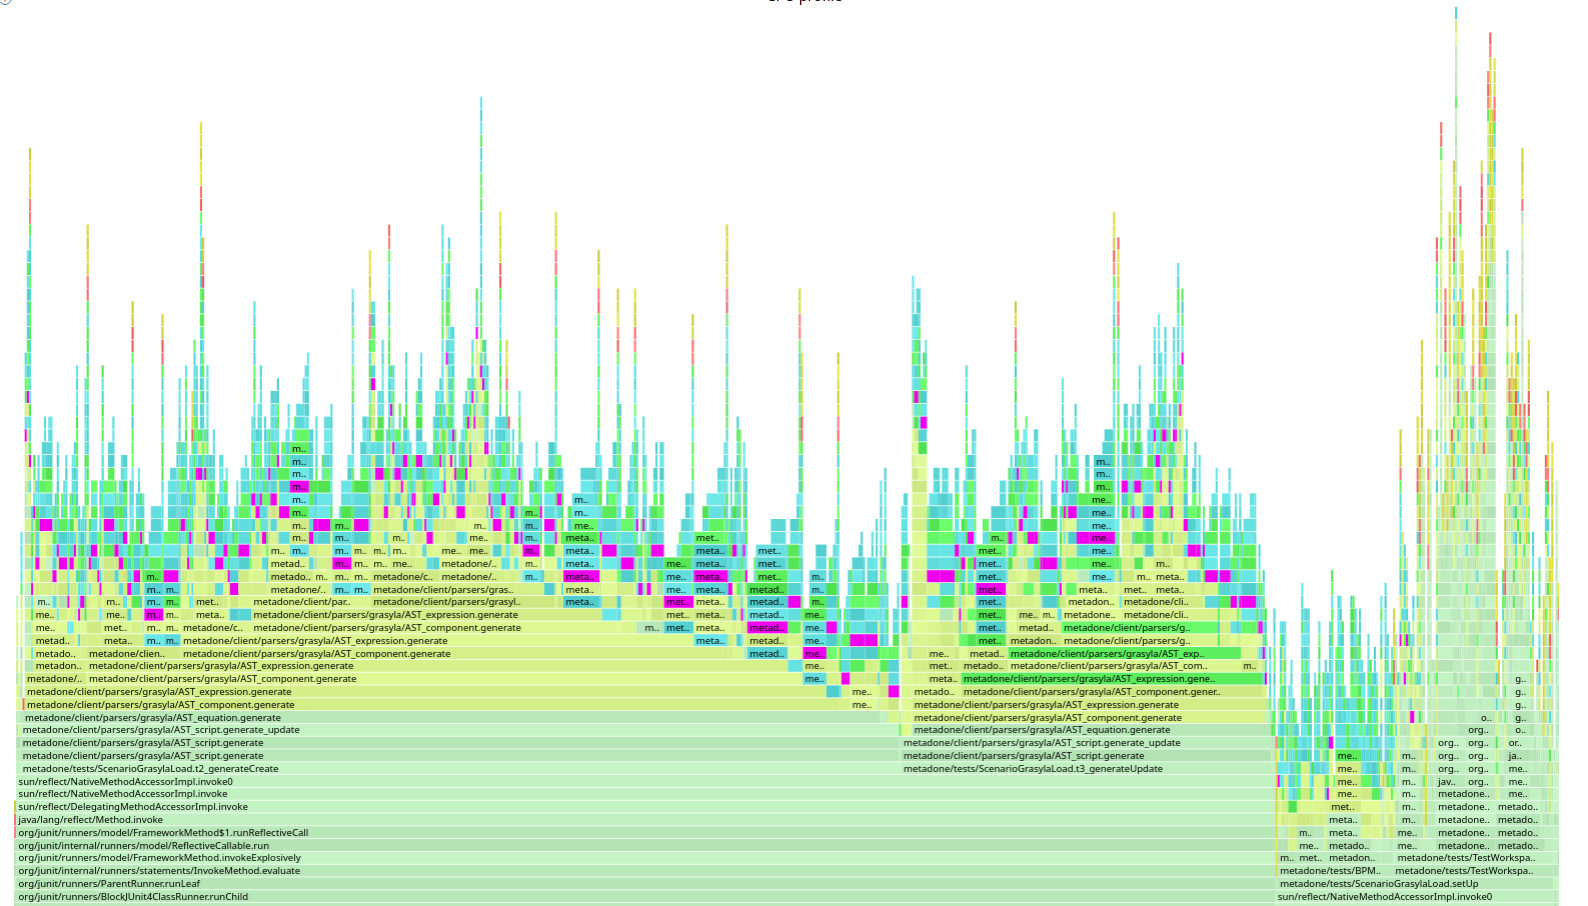
\includegraphics[width=0.9\textwidth]{img/createRole.png}
\caption{Flamegraph avec la fonction \texttt{ConcreteModel\_impl.\_createRole()} (bundle \texttt{metadone\_bundle\_metabusiness}) mise en évidence}
\label{fig:async-createRole}
\end{figure}
Le fait que \texttt{\_createRole()} représente 72\,\% du temps total, et que cette méthode soit appelée exclusivement depuis \texttt{AST\_expression.generate()} (76\,\%), indique que la quasi-totalité du temps de génération est consommée par les opérations d'écriture JPA, et non par la logique de traversée de l'AST ni par les vérifications de précondition.

À titre de comparaison, la méthode \texttt{getDefinitionRestricted()}, annotée du commentaire \texttt{// XXX horrible performance} dans le code source, ne représente que 0,14\,\% du temps d'exécution. Ce contraste illustre concrètement la nécessité de mesurer avant d'optimiser~: la fonction signalée comme problématique s'avère négligeable, tandis que le véritable goulot se situe ailleurs.

\subsection{Analyse du goulot : la persistance du ConcreteRole}
Le modèle de données de MetaDONE repose sur le méta-modèle MetaL$_2$, dans lequel tout est un objet, y compris les rôles concrets. Un \texttt{ConcreteRole} n'est pas un simple lien entre deux objets ; c'est lui-même une entité de premier rang, dotée d'une identité propre et susceptible de porter des propriétés ou d'être lui-même domaine ou range d'un autre rôle.

Cette décision architecturale se traduit directement dans la couche de persistance JPA. Chaque appel à \texttt{\_createRole()} exécute deux opérations d'insertion distinctes~:
\begin{lstlisting}[firstnumber=332,
  caption={Création du rôle avec \texttt{K\_Object} et \texttt{K\_Property} ---
  méthode \texttt{ConcreteModel\_impl.\_createRole()},
  bundle \texttt{metadone\_bundle\_metabusiness}.},
  label={ls-createRole}]
try {
    final K_PropertyType theMetaRole = mr.getMetaroleType();

    final K_Object result_o = mr.getTarget().createObject(); // INSERT #1 : K_Object
    theMetaRole.createProperty(result_o.getDataObject(), domain.getTarget(), range.getTarget()); // INSERT #2 : K_Property
    final ConcreteRole_impl result = FactoryOfProxy.buildConcreteRole(result_o);
    this.addInDefinition(result);
    return result;
}
\end{lstlisting}

\texttt{K\_Object} représente le \texttt{ConcreteRole} comme entité autonome dans la base. Il reçoit un identifiant unique (OID) et est stocké dans la table des objets. \texttt{K\_Property} représente le lien typé entre le domaine, le range et le \texttt{K\_PropertyType} correspondant au \texttt{MetaRole} qui gouverne ce lien.
Dans un modèle relationnel classique, un lien entre deux objets se réduirait à une ligne dans une table de jointure --- un seul INSERT. La généralité de MetaL$_2$ exige ici deux entités JPA par rôle, doublant mécaniquement le nombre d'opérations d'écriture. Pour un script de 106 équations dont chacune contient un arbre d'expressions potentiellement profond, ce surcoût se répercute sur des centaines à des milliers d'insertions lors d'une seule opération de chargement.

\subsection{Optimisations étudiées}
\label{sec:scenario2-opti}

Le goulot étant dans les INSERTs JPA eux-mêmes, toute amélioration significative devra agir à ce niveau. Une candidate locale a d'abord été examinée puis écartée~; trois pistes plus structurelles sont ensuite discutées.

\subsubsection{Court-circuit de la précondition (écartée)}
\label{sec:scenario2-precondition-rejet}

La méthode \texttt{precondition\_createRole()} vérifie, avant chaque création de rôle, que la cardinalité du \texttt{MetaRole} n'est pas violée. Pour la cardinalité \texttt{MANY\_TO\_MANY} --- utilisée notamment par les rôles liant chaque expression à ses éléments enfants --- la vérification consiste à parcourir l'ensemble des propriétés existantes depuis le domaine pour détecter d'éventuels doublons. Cette traversée est de complexité $O(N)$ par appel, soit $O(N^2)$ au total pour $N$ enfants d'un même nœud.

Cependant, le profileur positionne la précondition à moins de 1\,\% du temps d'exécution total. Deux facteurs expliquent ce résultat~: les collections JPA sont maintenues en mémoire dans l'identity map (la traversée est une itération Java pure, sans accès base), et le nombre d'enfants par nœud d'expression reste structurellement limité dans les scripts réels.

Au-delà du gain nul attendu, court-circuiter la précondition violerait le principe de \emph{Design by Contract} (section~\ref{sec:dbc}) qui est constitutif du design de MetaDONE~: chaque opération expose une postcondition garantie en échange du respect d'une précondition vérifiée. Supprimer cette vérification affaiblirait les garanties offertes par l'API et introduirait un risque de corruption silencieuse du modèle en cas d'appel incorrect. Cette piste cumulait donc deux raisons indépendantes de rejet --- absence de gain mesurable et incompatibilité avec les invariants architecturaux --- et a été définitivement écartée.

\subsubsection{Piste 1 — Mode de flush différé (FlushModeType.COMMIT)}


Par défaut, OpenJPA opère en mode FlushModeType.AUTO : il peut forcer une synchronisation avec la base avant toute requête susceptible de lire des données en attente d'écriture. En passant en mode FlushModeType.COMMIT pour la durée de generate(), tous les appels à em.persist() s'accumulent dans l'identity map sans écriture immédiate. La synchronisation n'a lieu qu'au commit de la transaction, ce qui permet à OpenJPA de regrouper l'ensemble des INSERTs en un seul batch JDBC — donnant ainsi à batchLimit une opportunité réelle de produire un effet, les insertions n'étant plus fragmentées par des flush intermédiaires.

La difficulté principale réside dans l'accès à l'EntityManager : celui-ci est encapsulé dans la couche repository JPA, tandis que generate() opère au niveau metabusiness. Exposer ou propager une référence à l'EntityManager jusqu'à ce niveau nécessite de traverser plusieurs couches d'abstraction et risque d'introduire un couplage architectural non souhaité.

\subsubsection{Piste 2 — Insertions JDBC directes}

Pour les phases de création en lot, il serait possible de contourner entièrement le cycle JPA et d'utiliser des PreparedStatement JDBC en mode batch pour insérer directement les enregistrements K\_Object et K\_Property. L'identity map JPA serait ensuite rafraîchie pour rester cohérente. Cette approche est théoriquement la plus efficace, car elle supprime l'intégralité de l'overhead JPA (dirty-checking, gestion des événements de cycle de vie, interception des proxies). Elle est également la plus risquée : elle rompt l'isolation de la couche persistance et exige une connaissance précise du schéma SQL généré par OpenJPA.

\subsubsection{Piste 3 — Révision du modèle de persistance du ConcreteRole}

Il s'agit de l'approche la plus fondamentale. Si, dans les cas d'utilisation courants, un \texttt{ConcreteRole} n'est jamais lui-même domaine ou range d'un autre rôle, il pourrait être représenté par une simple ligne dans une table de jointure plutôt que par deux entités JPA distinctes. Cette modification réduirait de moitié le nombre d'insertions et constituerait le gain le plus direct sur le goulot identifié. Elle remettrait cependant en question la généralité du méta-modèle MetaL$_2$ et représenterait un changement architectural majeur, dont les répercussions dépasseraient le cadre de ce scénario.

\subsection{Impact a posteriori d'Opt-5A sur le Scénario 2}
\label{sec:scenario2-opt5a}

Le diagnostic ci-dessus ayant identifié \texttt{\_createRole()} comme dominant
(72\,\% du CPU), il est naturel de questionner l'impact sur ce scénario de
l'optimisation \textbf{Opt-5A} développée pour le Scénario~5
(section~\ref{sec:scenario5}). Opt-5A modifie justement
\texttt{\_createRole()} en court-circuitant l'appel à \texttt{addInDefinition}
pour insérer directement dans le cache d'appartenance, ce qui élimine un
scan redondant interne à chaque création de rôle.

Deux campagnes complètes ont été menées (10 répétitions chacune,
mesures détaillées en annexe~\ref{ann:mesures-s2})~: une campagne
\emph{pré-Opt-5A} sur le code obtenu en revertant temporairement le
commit qui introduit l'optimisation, et une campagne \emph{post-Opt-5A}
sur le code intégrant Opt-5A. Les médianes obtenues sont rapportées au
tableau~\ref{tab:scenario2-opt5a}.

\begin{table}[h]
\centering
\caption{Scénario 2 avant et après Opt-5A. Médianes calculées sur 10
répétitions par campagne (mesures complètes en
annexe~\ref{ann:mesures-s2}).}
\label{tab:scenario2-opt5a}
\begin{tabular}{lrrr}
\hline
\textbf{Phase} & \textbf{Pré-Opt-5A} & \textbf{Post-Opt-5A} & \textbf{Gain} \\
\hline
t1 -- Parsing                & 17,78~ms (CV~3,9\,\%)    & 17,03~ms (CV~16,4\,\%) & $\approx$~1,0 \\
t2 -- Génération (création)  & 4\,170,35~ms (CV~1,1\,\%) & 571,76~ms (CV~2,3\,\%) & $\times$\,7,3 \\
t3 -- Génération (mise à jour) & 1\,739,91~ms (CV~4,1\,\%) & 291,54~ms (CV~12,5\,\%) & $\times$\,6,0 \\
t4 -- Traversée              & 2,30~ms (CV~14,8\,\%)    & 2,52~ms (CV~12,9\,\%) & $\approx$~1,0 \\
\hline
\end{tabular}
\end{table}

Le résultat est significatif sur les deux phases où la persistance domine~:
\textbf{$\times$\,7,3 sur la création} et \textbf{$\times$\,6,0 sur la
mise à jour}. Les phases t1 et t4, qui ne dépendent pas de
\texttt{\_createRole()}, restent inchangées comme attendu. Les
coefficients de variation très bas en pré-Opt-5A (1,1\,\% sur t2,
4,1\,\% sur t3) confirment que les gains observés sont robustes et ne
résultent pas d'un artefact de mesure.

Ce résultat n'invalide pas le diagnostic : le coût structurel des deux
insertions JPA par \texttt{ConcreteRole} reste réel et constitue toujours
le plancher des performances. Mais il révèle qu'une partie significative
du temps observé en S2 ne provenait pas de la persistance elle-même ---
le scan redondant intégré à \texttt{addInDefinition} ajoutait un surcoût
purement algorithmique, indépendant des INSERTs JPA. Opt-5A élimine ce
surcoût et ramène le temps de chargement à un ordre de grandeur
acceptable pour un script de 106 équations.

\subsection{Conclusion du scénario}
Le Scénario~2 illustre un cas dans lequel le goulot d'étranglement initial combine deux causes distinctes~: d'une part le coût structurel d'un choix de modélisation --- la représentation de chaque \texttt{ConcreteRole} comme une entité JPA autonome, conséquence directe de la généralité du méta-modèle MetaL$_2$ ---, d'autre part un surcoût algorithmique caché dans \texttt{addInDefinition} qui amplifiait artificiellement le coût de la persistance. Le diagnostic initial avait correctement localisé \texttt{\_createRole()} comme dominant sans pouvoir distinguer ces deux composantes.

L'analyse menée dans le Scénario~5 a permis d'isoler la seconde et de produire Opt-5A, dont l'impact collatéral sur le Scénario~2 ($\times$\,7,3 sur t2) est documenté ci-dessus. Le coût résiduel (572~ms pour 106~équations) reflète désormais le plancher structurel des deux INSERTs JPA par \texttt{ConcreteRole}~: il n'est plus accessible aux optimisations locales et son traitement passerait soit par une évolution de la couche de persistance (Pistes~1 et~2), soit par une révision du modèle de données (Piste~3), deux choix dont l'impact architectural dépasse le périmètre d'une optimisation locale.

%Ce scénario illustre par ailleurs une leçon méthodologique~: un goulot identifié dans un scénario peut combiner plusieurs causes que seul un autre scénario, abordé sous un angle différent, permet de séparer. La cohérence du cycle mesure--analyse--optimisation tient au fait que chaque diagnostic enrichit la compréhension globale, même lorsqu'aucune optimisation n'est implémentée localement.